%%%%%%%%%%%%%%%%%%%%%%%%%%%%%%%%%%%%%%%%%
% Short Sectioned Assignment LaTeX Template Version 1.0 (5/5/12)
% This template has been downloaded from: http://www.LaTeXTemplates.com
% Original author:  Frits Wenneker (http://www.howtotex.com)
% License: CC BY-NC-SA 3.0 (http://creativecommons.org/licenses/by-nc-sa/3.0/)
%%%%%%%%%%%%%%%%%%%%%%%%%%%%%%%%%%%%%%%%%

%----------------------------------------------------------------------------------------
%	PACKAGES AND OTHER DOCUMENT CONFIGURATIONS
%----------------------------------------------------------------------------------------

\documentclass[paper=a4, fontsize=11pt]{scrartcl} % A4 paper and 11pt font size

% ---- Entrada y salida de texto -----

\usepackage[T1]{fontenc} % Use 8-bit encoding that has 256 glyphs
\usepackage[utf8]{inputenc}
%\usepackage{fourier} % Use the Adobe Utopia font for the document - comment this line to return to the LaTeX default

% ---- Idioma --------

\usepackage[spanish, es-tabla]{babel} % Selecciona el español para palabras introducidas automáticamente, p.ej. "septiembre" en la fecha y especifica que se use la palabra Tabla en vez de Cuadro

% ---- Otros paquetes ----

\usepackage{url} % ,href} %para incluir URLs e hipervínculos dentro del texto (aunque hay que instalar href)
\usepackage{hyperref}
\hypersetup{
	colorlinks=true,
	linkcolor=black,
	urlcolor=black,
	citecolor=black,
}
\usepackage{amsmath,amsfonts,amsthm} % Math packages
%\usepackage{graphics,graphicx, floatrow} %para incluir imágenes y notas en las imágenes
\usepackage{graphics,graphicx, float} %para incluir imágenes y colocarlas

% Para hacer tablas comlejas
%\usepackage{multirow}
%\usepackage{threeparttable}

%\usepackage{sectsty} % Allows customizing section commands
%\allsectionsfont{\centering \normalfont\scshape} % Make all sections centered, the default font and small caps

\usepackage{fancyhdr} % Custom headers and footers
\pagestyle{fancyplain} % Makes all pages in the document conform to the custom headers and footers
\fancyhead{} % No page header - if you want one, create it in the same way as the footers below
\fancyfoot[L]{} % Empty left footer
\fancyfoot[C]{} % Empty center footer
\fancyfoot[R]{\thepage} % Page numbering for right footer
\renewcommand{\headrulewidth}{0pt} % Remove header underlines
\renewcommand{\footrulewidth}{0pt} % Remove footer underlines
\setlength{\headheight}{13.6pt} % Customize the height of the header

\numberwithin{equation}{section} % Number equations within sections (i.e. 1.1, 1.2, 2.1, 2.2 instead of 1, 2, 3, 4)
\numberwithin{figure}{section} % Number figures within sections (i.e. 1.1, 1.2, 2.1, 2.2 instead of 1, 2, 3, 4)
\numberwithin{table}{section} % Number tables within sections (i.e. 1.1, 1.2, 2.1, 2.2 instead of 1, 2, 3, 4)

\setlength\parindent{0pt} % Removes all indentation from paragraphs - comment this line for an assignment with lots of text

\newcommand{\horrule}[1]{\rule{\linewidth}{#1}} % Create horizontal rule command with 1 argument of height
\usepackage{booktabs}

\usepackage{listings}
\lstdefinelanguage
[x64]{Assembler}     % add a "x64" dialect of Assembler
[x86masm]{Assembler} % based on the "x86masm" dialect
{morekeywords={CDQE,CQO,CMPSQ,CMPXCHG16B,JRCXZ,LODSQ,MOVSXD, %
		POPFQ,PUSHFQ,SCASQ,STOSQ,IRETQ,RDTSCP,SWAPGS, %
		rax,rdx,rcx,rbx,rsi,rdi,rsp,rbp, %
		r8,r8d,r8w,r8b,r9,r9d,r9w,r9b, %
		r10,r10d,r10w,r10b,r11,r11d,r11w,r11b, %
		r12,r12d,r12w,r12b,r13,r13d,r13w,r13b, %
		r14,r14d,r14w,r14b,r15,r15d,r15w,r15b}} % etc.
\usepackage{color}
\usepackage{xcolor}
\lstdefinestyle{customc}{
	belowcaptionskip=1\baselineskip,
	breaklines=true,
	frame=L,
	xleftmargin=\parindent,
	language=C,
	showstringspaces=false,
	basicstyle=\footnotesize\ttfamily,
	keywordstyle=\bfseries\color{green!40!black},
	commentstyle=\itshape\color{purple!40!black},
	identifierstyle=\color{blue},
	stringstyle=\color{orange},
}

\lstset{escapechar=@,style=customc}
\usepackage{url}

\title{	
	\normalfont \normalsize
	\begin{figure}[htb]
		\centering
		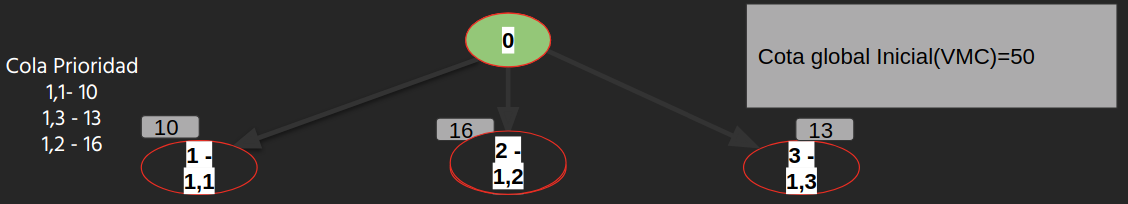
\includegraphics[width=0.3\textwidth]{./imagenes/1}
	\end{figure}
	\textsc{\textbf{Algoritmica} \\ Grado en Ingeniería Informática \\ 
	Curso 2018-2019} \\ [25pt] 
	\begin{figure}[htb]
		\centering
		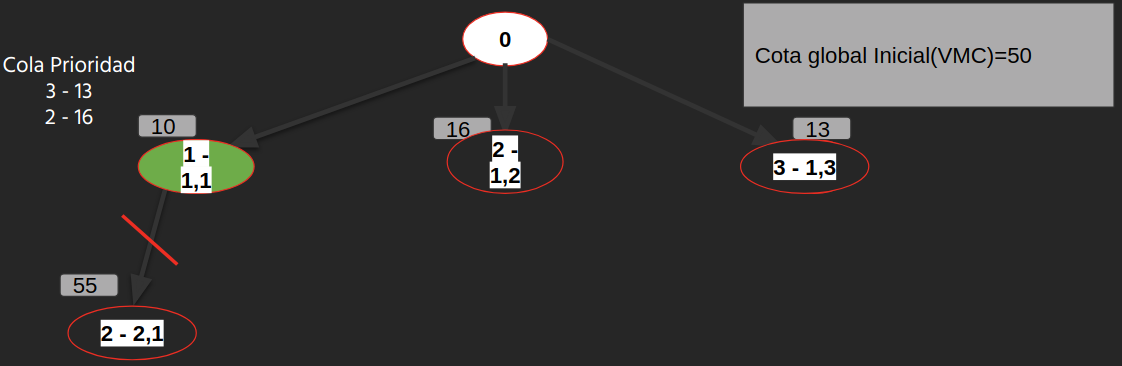
\includegraphics[width=0.15\textwidth]{./imagenes/2}
	\end{figure}
	\horrule{0.5pt} \\[0.4cm]
	\huge Ejercicio Propuesto. \\
	\huge Mochila 0-1
	\\ 
	\horrule{2pt} \\[0.5cm] 
}
\author{Félix Ramírez García  \\
\href{mailto:felixramirezgarcia@correo.ugr.es}{felixramirezgarcia@correo.ugr.es}}
\date{\normalsize\today} 

%----------------------------------------------------------------------------------------
% DOCUMENTO
%----------------------------------------------------------------------------------------

\begin{document}
	
	\maketitle % Muestra el Título
	
	\newpage %inserta un salto de página
	
	\tableofcontents % para generar el índice de contenidos
	
	\listoffigures % para generar índice de imágenes.
	
	\listoftables % para generar índice de tablas.
	
	\newpage
	
	%-----------------------------------------------------------------------
	%							Introduccion
	%----------------------------------------------------------------------	
	\section[Introducción]{Introducción}

	 Supongamos que tenemos n distintos tipos de ítems, que van de 1 a n. De cada tipo de ítem se tiene solamente un ítem disponible. \\
	
	Cada tipo de ítem i tiene un beneficio asociado dado por vi y un peso (o volumen) wi. Usualmente se asume que el beneficio y el peso no son negativos. Para simplificar la representación, se suele asumir que los ítems están listados en orden creciente según el peso (o volumen). \\
	
	Por otro lado se tiene una mochila, donde se pueden introducir los ítems, que soporta un peso máximo (o volumen máximo) W. \\
	
	El problema consiste en meter en la mochila ítems de tal forma que se maximice el valor de los ítems que contiene y siempre que no se supere el peso (o volumen) máximo que puede soportar la misma. La solución al problema vendrá dado por la secuencia de variables x1, x2, ..., xn donde el valor de xi (0-1) indica si existe en la mochila el ítem del tipo i. \\
	
	%-----------------------------------------------------------------------
	%							Solucion fuerza bruta
	%----------------------------------------------------------------------	
	\section[Solución fuerza bruta]{Solución fuerza bruta}

	
	\lstset{language=C}
	\begin{lstlisting}[frame=single]

	\end{lstlisting} 
	
	%-----------------------------------------------------------------------
	%							Solucion con backtraking
	%----------------------------------------------------------------------	
	\section[Solución con backtraking]{Solución con backtraking}

	
	\lstset{language=C}
	\begin{lstlisting}[frame=single]

	\end{lstlisting} 

	%-----------------------------------------------------------------------
	%							Estudio empirico de la eficiencia
	%----------------------------------------------------------------------	
	\section[Estudio empírico de la eficiencia]{Estudio empírico de la eficiencia}
		
	Tras la ejecución del programa de fuerza bruta se han obtenido los siguientes resultados, donde la primera columna es el tamaño y la segunda el tiempo:\\
	
	\lstset{language=C}
	\begin{lstlisting}[frame=single]

	\end{lstlisting} 
	
	La gráfica obtenida con las salidas de fuerza bruta se muestra en la figura xx: \\
	
		%\begin{figure}[htb]
		%	\centering
		%	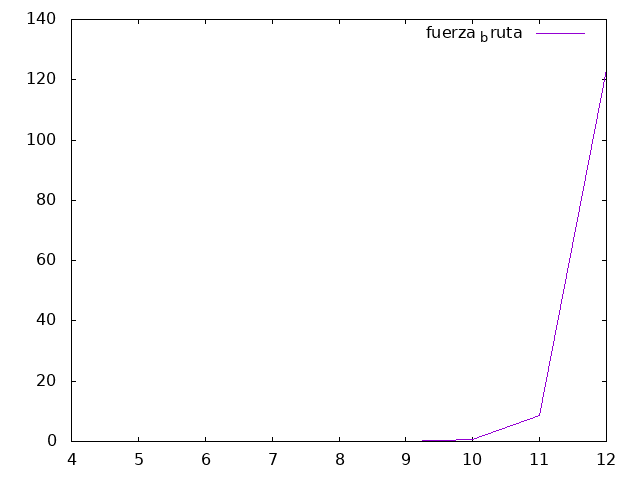
\includegraphics[width=0.8\textwidth]{./imagenes/fuerza_bruta}
		%	\caption{Fuerza bruta} \label{fig:1}
		%\end{figure}
	
	Tras la ejecución del programa con backtraking se han obtenido los siguientes resultados, donde la primera columna es el tamaño y la segunda el tiempo: \\
	
	\lstset{language=C}
	\begin{lstlisting}[frame=single]

	\end{lstlisting} 

	La gráfica obtenida con las salidas de backtraking se muestra en la figura 4.2: \\

	%\begin{figure}[htb]
	%	\centering
	%	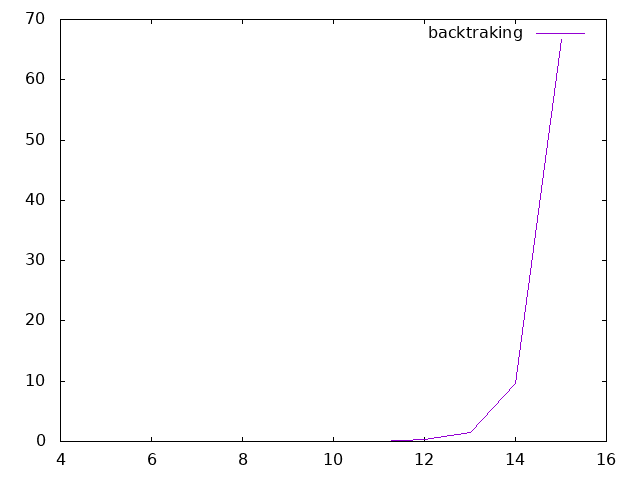
\includegraphics[width=0.8\textwidth]{./imagenes/backtraking}
	%	\caption{Fuerza bruta} \label{fig:1}
	%\end{figure}
	


	%-----------------------------------------------------------------------
	%							BIBLIOGRAFIA
	%-----------------------------------------------------------------------
	% Referencia a bibliografia			En \cite{Baz}
	% Referencia a figura				La figura (\ref{fig:1})
	% Espacio entre lineas				\vspace{0.06in}
	% Figura con comentario al pie
	%\begin{figure}[htb]
	%	\centering
	%	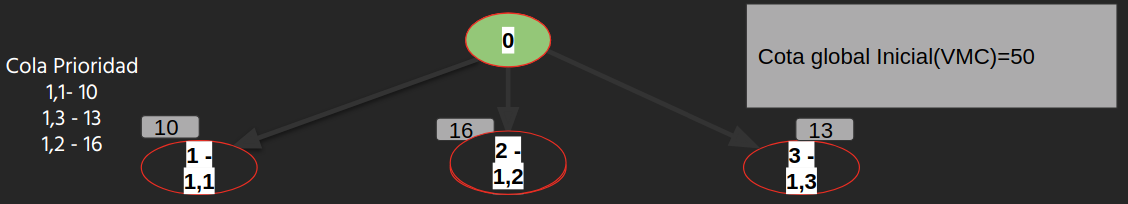
\includegraphics[width=0.4\textwidth]{./imagenes/1}
	%	\caption{Universidad de Granada.} \label{fig:1}
	%\end{figure}
	%\begin{thebibliography}{99}
	%	\bibitem{Baz} 
	%	\textsc{Bazaraa, M.S., J.J. Jarvis}
	%	\textit{Programacuib}.
	%	\newline
	%	\url{https://www.google.es}	
	%\end{thebibliography}

	


\end{document}